%%
% このファイルは筑波大学情報学群情報科学類の卒業研究論文のサンプルです。
% このファイルを書き換えて、このサンプルと同様の書式の論文をLaTeXを使って
% 作成できます。
% 
% OSやLaTeXの設定によっては漢字コードや改行コードを変更する必要があります。
%%
\documentclass[a4paper,11pt]{jreport}

%%\usepackage[dvipdfmx,bookmarks=true,bookmarksnumbered=true,bookmarkstype=toc]{hyperref} \usepackage{pxjahyper}
%%\usepackage{ulem}
\usepackage[dvipdfmx]{graphicx} % for \includegraphics[width=3cm]{sample.pdf}
\usepackage{times} % use Times Font instead of Computer Modern
\usepackage{ulem}

\setcounter{tocdepth}{3}
\setcounter{page}{-1}

\setlength{\oddsidemargin}{0.1in}
\setlength{\evensidemargin}{0.1in}
\setlength{\topmargin}{0in}
\setlength{\textwidth}{6in}
%\setlength{\textheight}{10.1in}
\setlength{\parskip}{0em}
\setlength{\topsep}{0em}

%% タイトル生成用パッケージ(重要)
\usepackage{coins-jp}

%% タイトル
\title{差分プライバシー保証のための汎用プログラミングフレームワークの設計}
%% 著者
\author{筑波 太郎}
%% 指導教員
\advisor{筑波 大二郎}

%% 年度と主専攻名
\fiscalyear{2022}
\majorfield{情報システム主専攻}

\begin{document}
\maketitle
\thispagestyle{empty}
\newpage

\thispagestyle{empty}
\vspace*{20pt plus 1fil}
\parindent=1zw
\noindent
%%
%% 論文の要旨
%%
\begin{center}
{\Large \textbf 要旨}
\vspace{2cm}
\end{center}
この文書は筑波大学情報学群情報科学類の卒業研究論文のサンプルである。
このファイルを書き換えて、このサンプルと同様の書式の論文を \LaTeX を
使って作成できる。

このサンプルは、学生が論文を作成する手間を軽減するために提供している。
このサンプルで示す書式はあくまで例であり、要項に準拠していれば、この
ファイルを使わずに自分で決めた書式を用いてもよい。

%%%%%
\par
\vspace{0pt plus 1fil}
\newpage

\pagenumbering{roman} % I, II, III, IV 
\tableofcontents
\listoffigures
%\listoftables

\pagebreak \setcounter{page}{1}
\pagenumbering{arabic} % 1,2,3

\chapter{序論}

情報化が進んだ現代で、個人情報を含むデータへのプライバシー保護が重要になっている。
しかし、アプリケーションの脆弱性を突いた攻撃や情報漏洩を目的としたマルウェアへの感染、複数のデータベースを組み合わせ共通している列を見つけ出す、
匿名化していてもその情報の組み合わせを持つ人が1人しか居ないなど、様々な手法でk匿名性が破れ個人情報は漏洩してしまう。

それらの対策として、差分プライバシー技術が存在する。
これは、データに特定個人が存在する場合としない場合の統計結果が区別できないようなノイズを載せる手法である。
これを用いて個人情報の漏洩を防止する。
ノイズの実現方法の例としては、ラプラス分布やガウシアン分布が挙げられる。
これによりノイズが載っていても”尤もらしい”データを出力することができる。

しかし、既存の差分プライバシー技術は複雑な統計処理が困難という問題がある。
そのため本研究では、任意の演算を行い複雑な統計処理と差分プライバシーの両立を実現することが目的である。
この研究により、新たに複雑な統計処理が実現可能となる。

\section{関連研究}

差分プライバシーを用いた既存研究では、Royce J Wilsonらによる先行研究がある。
これは、差分プライバシーを適用した状態でApache Sparkなどの分散データ処理を行うデータベースにアクセスするSQLの提案である。
この研究の成果としてGoogleの多言語差分プライバシーライブラリであるDifferential PrivacyやOpenMindによるPipelineDPが開発された。
信用できないクライアントからデータベースに対してクエリを投げると差分プライバシー適用済みで結果が返ってくる仕組みである。
これはSQLが実現できる範囲で統計を処理する場合に有用である。

\subsection{問題点}

一方、統計結果を前提に別の統計結果を実行したり、生のデータを利用した深層学習などはできない。

またSQLの関係代数で表現できない演算は行えない、できてもクエリが複雑になるといった問題がある。
例としては、2次元ではない多次元に対する平均や最頻値の処理、データを元に機械学習を行いそのネットワークを出力する処理、
値を丸め込んだり数値ではなくnビットの情報量(都道府県など)を扱いたい場合が挙げられる。

\section{提案手法}

\begin{figure}[htbp]
    \centering
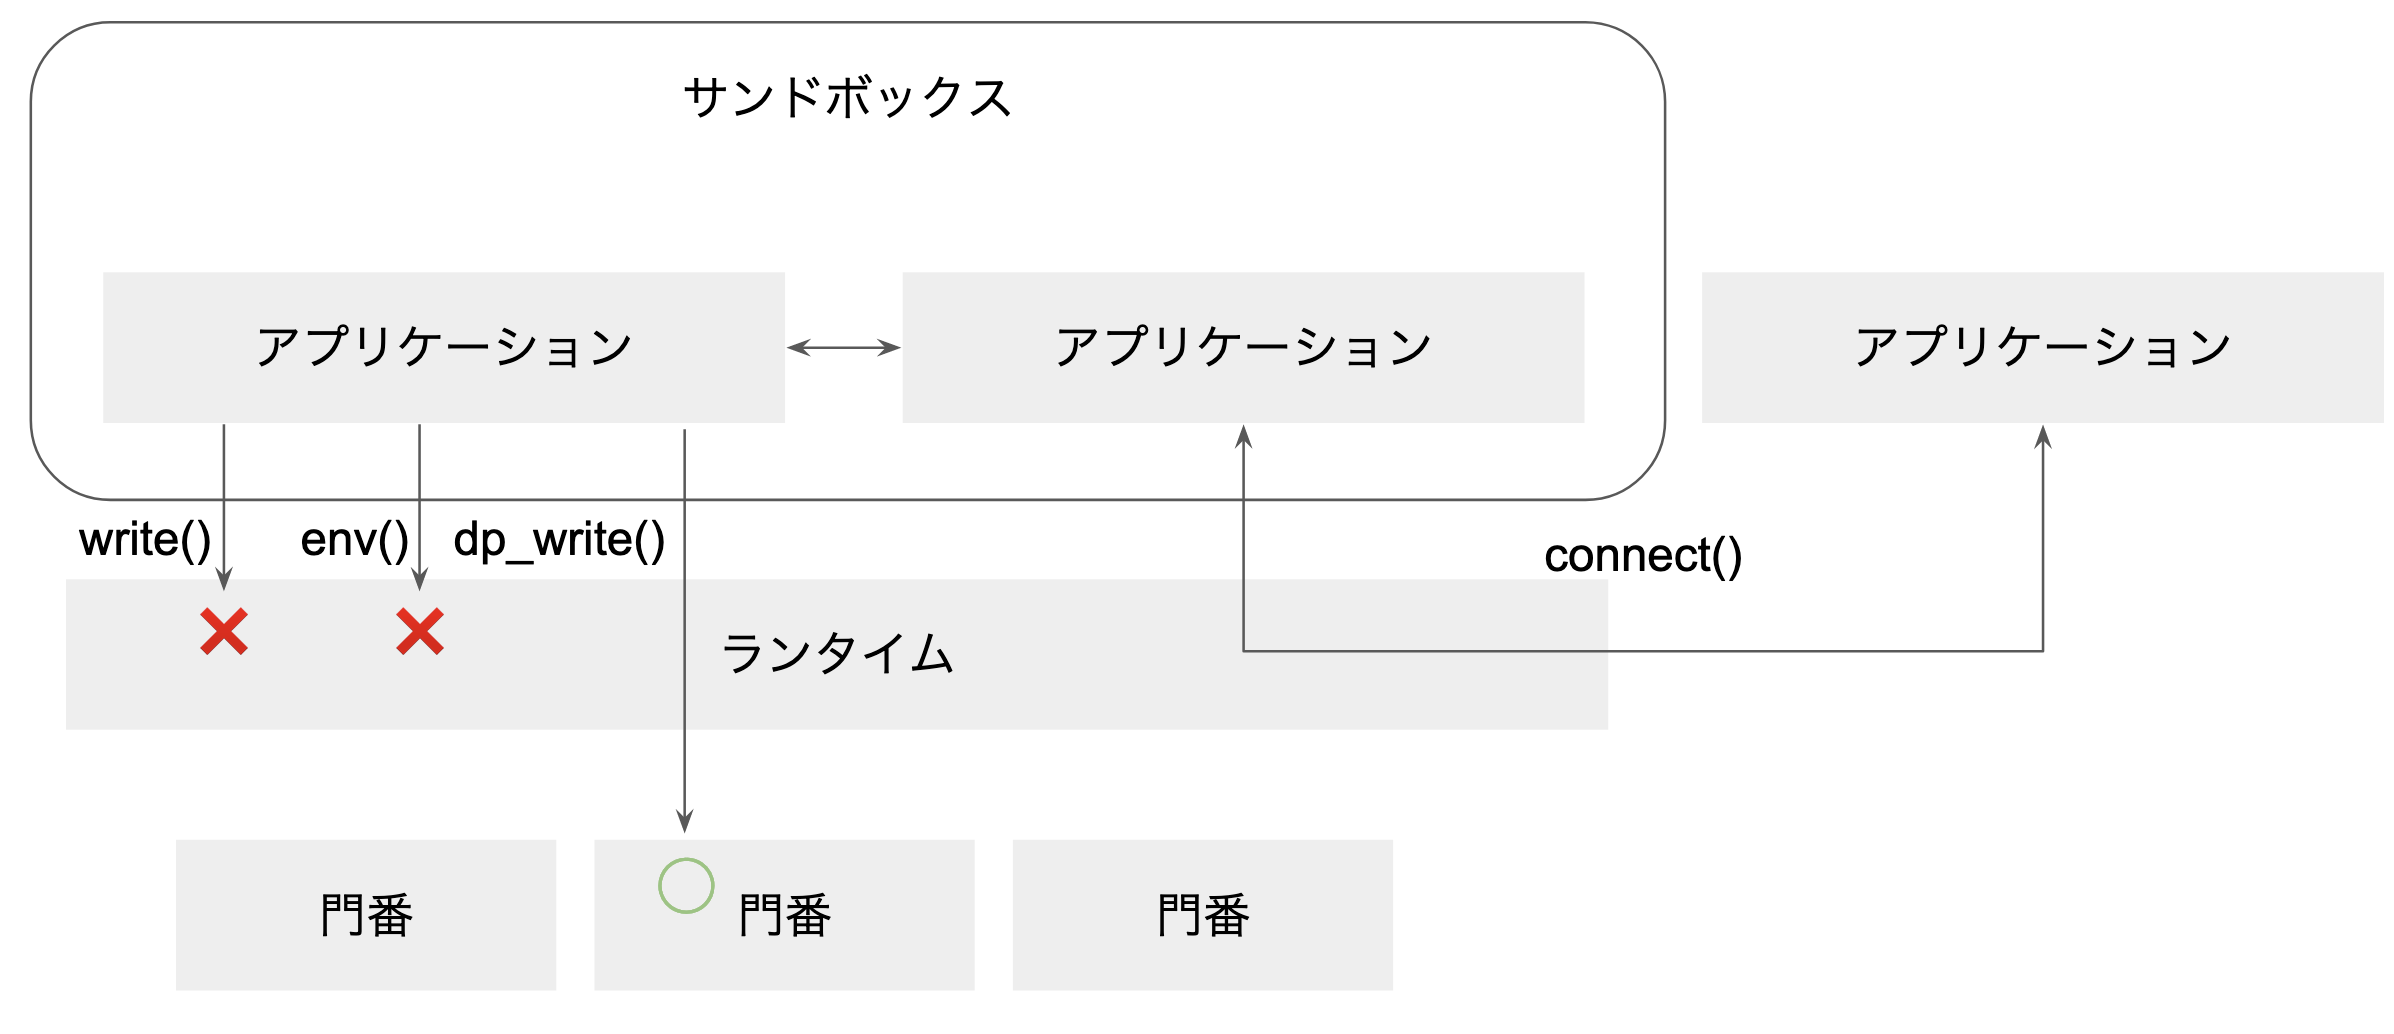
\includegraphics[height=50mm]{architecture.png}
    \caption{フレームワークのアーキテクチャ}
    \label{fig:architecture}
\end{figure}

\subsection{サンドボックス}

この研究では、任意の仮想的な計算機(=サンドボックス)を用いて、サンドボックス型のフレームワークを開発・評価することで、任意のプログラムの実行を可能にし幅広い統計処理を実現する。
サンドボックス技術としてWebAssmeblyを検討している。
任意の言語で書かれたプログラムを、コンパイラでWebAssembly形式にコンパイルし独自のランタイムで実行する。
WebAssemblyはWebブラウザ向けに開発された中間言語で、あらかじめさまざまな言語からコンパイルされたバイナリ形式のファイルをランタイムが動くさまざまな環境で動作させることができる技術である。
本フレームワークでは、サンドボックスを利用することで、内部では差分プライバシーに対応した出力を行えるシステムコールのみ許可し、通常のファイル読み書きやネットワーク接続の禁止や条件付き許可を行う。
プログラムからプライバシーを守りつつ内部では統計処理を自由に行うことができる。(図\ref{fig:architecture})

\subsection{ライブラリ}

本フレームワークの一部として各言語用にライブラリ・ラッパーを提供し、差分プライバシーを用いた出力を行う際も出力する関数を置き換えるだけなど、プログラムの変更が必要最低限に抑えられるようにする。

\subsection{門番}

サンドボックスが出力した生のデータは、信頼できる差分プライバシー計算機(=門番)が統計処理を行うこととする。
また出力形式としては、平均値や中央値、標準偏差や信頼区間、分散や総和を想定している。

\subsection{ノイズ処理}
本研究では、差分プライバシー技術を適用しながらも複雑な統計処理を実現するために、新たな手法を提案する。
それには、実現したい統計処理のデータ幅や偏差に適したノイズを生成し、統計結果が区別できない程度にだけノイズを加える。

\subsection{ノイズ手法}

出力する値にノイズを乗せる手法として、差分プライバシー技術を用いる。
サンドボックス内部のプログラムは、統計値に対して出力したい値、例えば平均値や合計値を直接計算せずに、門番に対してベクトル値をその計算種類を与える。
門番は、そのベクトル値から実際の合計値・平均値を計算する。その後ベクトル値のばらつきから偏差を求めて、ガウス分布にそう乱数を生成し、それを結果に対して加算する。
これにより、統計値にはガウス分布に従うノイズが加算される。
分布関数の裾野の大きさを、あらかじめ設定することで、ノイズの乗った値から真の値を見つける難易度を設定することができる。

\subsection{サンドボックス}

今回使用するサンドボックスは、前述するようにWebAssembly技術を用いている。
既存ランタイムであるWasmerのライブラリを用いて、新たな名前空間に差分プライバシー専用のシステムコールを追加する形でランタイムを構築した。
サンドボックス内部の

\section{現在の進捗状況}

差分プライバシーに対応したサンドボックスをWebAssemblyランタイムを用いて開発した。門番としてラプラス分布ノイズから平均値を出力することができる。
また簡易的なベンチマークを行えるように、LINPACKなどの数学計算プログラムを本たんライム用にコンパイルした。

\section{本システムの想定動作環境}
\section{評価}
\subsection{実験手法}
本研究で提案する手法を実験により評価する。

\subsection{差分プライバシーでの出力比較}
まず、差分プライバシーを適用した統計処理の結果と、それに対してノイズを加えなかった統計処理の結果を比較することで、本研究で提案する手法が有効であるかを確認する。

\subsection{計算時間の測定}
次に、差分プライバシーを適用した場合の計算時間の増加を測定する。
- 門番を使った場合と使ってない場合のオーバーヘッドが、定数時間で増えるかどうか
    - データ量を増やして複数やってみる

- 他の言語でも書いてみる
- バジェットについての話

\section{結果}
\subsection{差分プライバシーでの出力比較}

\subsection{計算時間の測定}

\section{}
どういうふうに応用できるか

\section{結論}
本研究では、差分プライバシーを適用しながらも複雑な統計処理を実現するための新たな手法を提案した。
それにより、個人情報を含むデータに対するプライバシー保護を実現することができるだけでなく、新たに複雑な統計処理が実現可能となる。

\chapter*{謝辞}
\addcontentsline{toc}{chapter}{\numberline{}謝辞}

\newpage

\addcontentsline{toc}{chapter}{\numberline{}参考文献}
\renewcommand{\bibname}{参考文献}

%% 参考文献に jbibtex を使う場合
%\bibliographystyle{junsrt}
%\bibliography{samplebib}
%% [compile] jbibtex sample; platex sample; platex sample;

%% 参考文献を直接ファイルに含めて書く場合
\begin{thebibliography}{1}
\bibitem{Bibunsho}
奥村 晴彦, 黒木 裕介.
\newblock LaTeX2ε美文書作成入門 改訂第7版.
\newblock 技術評論社, 2017.

\bibitem{ScienceResearchWriting}
Hilary Glasman-Deal.
\newblock Science Research Writing: A Guide for Non-Native Speakers of English.
\newblock Imperial College Press, 2009.
\end{thebibliography}

\end{document}
